\section{Results}
\label{sec:results}

Our longitudinal evaluation generated 38 distinct execution traces across a four-week period. We present the findings organized by our three research questions, supported by statistical analysis (Mann-Kendall trend tests, Spearman correlations, and bootstrap confidence intervals).

\subsection{RQ1: Effectiveness of the Quality Gate}
The framework proved effective at enforcing release discipline. Of 38 evaluation runs, 36 received a PROMOTE decision and 2 were flagged as ROLLBACK (Table~\ref{tab:decision_log}). The two ROLLBACK decisions occurred during Run 1 and Run 2 (the first two evaluations in the longitudinal series), where evidence coverage dropped to 50\%---well below the 56\% ROLLBACK threshold (70\% of the 80\% target). This early detection prevented a build with inadequate citation behavior from being promoted in the staging gate.

While unit and integration tests confirmed API contracts and logic flow, the persona-grounded and multi-turn question bank evaluation isolated contextual errors that escaped traditional CI: hallucinating non-existent features, losing conversational context across multi-turn interactions, and providing unsupported claims without evidence citations. In practice, this pre-production simulation of customer-like usage accelerated iteration by exposing high-impact conversational failures earlier in the cycle. Beyond pre-production evaluation, the gate's structured feedback---particularly per-category issue labels and failure traces---also guided iterative agent development itself, directing engineering effort toward the specific error classes (e.g., hallucination, evidence gaps) that the gate surfaced across runs.

Over the four-week evaluation spanning 20+ internal releases, no promoted build subsequently triggered a rollback in later runs, indicating stable post-promote behavior under the gate's criteria.

\begin{table*}[htbp]
\renewcommand{\arraystretch}{1.2}
\centering
\small
\setlength{\tabcolsep}{3.5pt}
\caption{Complete evaluation trace results across 38 runs with 5 quality dimensions (Task Success Rate consolidates the legacy Success/Helpful overlap).}
\label{tab:decision_log}
\begin{tabular}{rrrrrrrl}
\toprule
\textbf{Run} & \textbf{Tests} & \textbf{Task Success} & \textbf{P95 (ms)} & \textbf{Context} & \textbf{Safety} & \textbf{Evidence} & \textbf{Decision} \\
\midrule
1 & 59 & 100.0\% & 8487 & 100\% & 97.0\% & 50\% & \textbf{ROLLBACK} \\
2 & 59 & 100.0\% & 12316 & 100\% & 97.0\% & 50\% & \textbf{ROLLBACK} \\
3 & 59 & 98.3\% & 7970 & 100\% & 97.0\% & 100\% & PROMOTE \\
4 & 13 & 100.0\% & 11522 & 100\% & 100.0\% & 100\% & PROMOTE \\
5 & 59 & 100.0\% & 9401 & 100\% & 97.0\% & 100\% & PROMOTE \\
6 & 13 & 100.0\% & 12397 & 100\% & 100.0\% & 100\% & PROMOTE \\
7 & 59 & 100.0\% & 9850 & 100\% & 97.0\% & 100\% & PROMOTE \\
8 & 59 & 100.0\% & 9089 & 100\% & 97.0\% & 100\% & PROMOTE \\
9 & 59 & 100.0\% & 10523 & 100\% & 97.0\% & 100\% & PROMOTE \\
10 & 59 & 100.0\% & 11593 & 100\% & 97.0\% & 100\% & PROMOTE \\
11 & 59 & 100.0\% & 12395 & 100\% & 97.0\% & 100\% & PROMOTE \\
12 & 86 & 94.2\% & 12095 & 100\% & 97.0\% & 100\% & PROMOTE \\
13 & 86 & 95.3\% & 14104 & 100\% & 97.0\% & 100\% & PROMOTE \\
14 & 86 & 97.7\% & 12124 & 100\% & 97.0\% & 100\% & PROMOTE \\
15 & 86 & 97.7\% & 11961 & 100\% & 97.0\% & 100\% & PROMOTE \\
16 & 86 & 100.0\% & 9617 & 100\% & 97.0\% & 100\% & PROMOTE \\
17 & 86 & 98.8\% & 11291 & 100\% & 97.0\% & 100\% & PROMOTE \\
18 & 86 & 100.0\% & 8422 & 100\% & 97.0\% & 100\% & PROMOTE \\
19 & 86 & 97.7\% & 10843 & 100\% & 97.0\% & 100\% & PROMOTE \\
20 & 86 & 98.8\% & 11393 & 100\% & 97.0\% & 100\% & PROMOTE \\
21 & 88 & 95.5\% & 11548 & 100\% & 98.0\% & 100\% & PROMOTE \\
22 & 88 & 94.3\% & 8756 & 100\% & 98.0\% & 100\% & PROMOTE \\
23 & 88 & 98.9\% & 11911 & 100\% & 98.0\% & 100\% & PROMOTE \\
24 & 88 & 100.0\% & 11661 & 100\% & 98.0\% & 100\% & PROMOTE \\
25 & 106 & 93.4\% & 12483 & 100\% & 96.0\% & 100\% & PROMOTE \\
26 & 106 & 97.2\% & 12096 & 100\% & 96.0\% & 100\% & PROMOTE \\
27 & 106 & 91.5\% & 12336 & 100\% & 96.0\% & 100\% & PROMOTE \\
28 & 106 & 96.2\% & 12291 & 100\% & 96.0\% & 100\% & PROMOTE \\
29 & 106 & 96.2\% & 13074 & 100\% & 96.0\% & 100\% & PROMOTE \\
30 & 106 & 98.1\% & 11669 & 100\% & 96.0\% & 100\% & PROMOTE \\
31 & 50 & 98.0\% & 8915 & 100\% & 96.0\% & 100\% & PROMOTE \\
32 & 106 & 100.0\% & 11762 & 100\% & 96.0\% & 100\% & PROMOTE \\
33 & 106 & 99.1\% & 11619 & 100\% & 96.0\% & 100\% & PROMOTE \\
34 & 133 & 95.5\% & 14116 & 100\% & 97.0\% & 90\% & PROMOTE \\
35 & 83 & 96.4\% & 14182 & 100\% & 98.0\% & 86\% & PROMOTE \\
36 & 83 & 96.4\% & 14631 & 100\% & 98.0\% & 86\% & PROMOTE \\
37 & 83 & 96.4\% & 14331 & 100\% & 98.0\% & 100\% & PROMOTE \\
38 & 133 & 98.5\% & 13833 & 100\% & 97.0\% & 100\% & PROMOTE \\
\bottomrule
\end{tabular}
\setlength{\tabcolsep}{6pt}
\end{table*}


\subsection{RQ1.1: Ablation Against Simplified Gates}
To estimate the practical value of each gate dimension, we ran an offline ablation over the same 38 runs (Table~\ref{tab:gate_ablation}). Removing evidence coverage from the decision logic would have promoted both severe failures that the full gate correctly rolled back. In contrast, the full five-dimension gate promoted zero severe-failure runs. A ``traditional CI only'' baseline (without behavioral gate) would have promoted all runs, including severe failures.

\begin{table}[htbp]
\renewcommand{\arraystretch}{1.2}
\centering
\scriptsize
\setlength{\tabcolsep}{2.5pt}
\caption{Gate ablation analysis across 38 runs with the consolidated 5D gate. Severe-promoted counts indicate missed critical failures (lower is better).}
\label{tab:gate_ablation}
\begin{tabular}{p{1.7cm}rrrr}
\toprule
\textbf{Scenario} & \textbf{Promote} & \textbf{Hold} & \textbf{Rollback} & \textbf{Sev.} \\
\midrule
Full 5D Gate & 36 & 0 & 2 & 0 \\
No Evidence Coverage & 38 & 0 & 0 & 2 \\
No Safety Dimension & 36 & 0 & 2 & 0 \\
Task Success + Latency Only & 38 & 0 & 0 & 2 \\
Traditional CI only (no behavioral gate) & 38 & 0 & 0 & 2 \\
\bottomrule
\end{tabular}
\setlength{\tabcolsep}{6pt}
\end{table}


\subsection{RQ2: Predictive Dimensions of Quality}

\begin{table}[htbp]
\renewcommand{\arraystretch}{1.2}
\centering
\small
\setlength{\tabcolsep}{3pt}
\caption{Spearman rank correlation matrix between variable quality dimensions (RC excluded as constant). $^{*}$\,$p<0.05$ (two-sided, $n=38$); coefficients without a marker are not statistically significant.}
\label{tab:correlations}
\begin{tabular}{lrrrr}
\toprule
 & \textbf{TaskSR} & \textbf{P95} & \textbf{Safety} & \textbf{Evid} \\
\midrule
\textbf{TaskSR} & 1.00 & -0.47$^{*}$ & 0.16 & 0.02 \\
\textbf{P95} & -0.47$^{*}$ & 1.00 & 0.03 & -0.27 \\
\textbf{Safety} & 0.16 & 0.03 & 1.00 & -0.20 \\
\textbf{Evid} & 0.02 & -0.27 & -0.20 & 1.00 \\
\bottomrule
\end{tabular}
\setlength{\tabcolsep}{6pt}
\end{table}


Spearman rank correlation analysis (Table~\ref{tab:correlations}) reveals the inter-dimensional structure of the consolidated five-dimension gate:
\begin{itemize}
    \item \textbf{Task Success Rate and P95 Latency} show moderate negative correlation ($\rho = -0.47$), indicating that slower responses tend to accompany lower quality, consistent with multi-agent timeout and retry failures degrading both dimensions simultaneously.
    \item \textbf{Evidence Coverage} was responsible for both ROLLBACK decisions (50\% vs.\ 80\% threshold), making it the most actionable predictor of severe regression. Correlation analysis therefore reinforces that citation-grounding failures, not the consolidated task-success construct, were the main severe-failure driver in this dataset.
    \item \textbf{Safety Pass Rate} remained consistently high ($\mu = 97.1\%$, 95\% CI $[96.8, 97.4]$) but showed no significant trend, serving as a stable baseline constraint.
    \item \textbf{Research Context Preservation} was excluded from correlation analysis because it remained constant at 100\% across all 38 runs under the deterministic context-enrichment pipeline. In this dataset it has no discriminative power, but it remains useful as a regression sentinel for future pipeline changes.
\end{itemize}

Bootstrap confidence intervals are reported in Table~\ref{tab:confidence_intervals} to contextualize central-tendency estimates with sampling uncertainty.
\begin{table}[htbp]
\renewcommand{\arraystretch}{1.2}
\centering
\small
\setlength{\tabcolsep}{3pt}
\caption{Bootstrap 95\% confidence intervals for metric means (B=10{,}000).}
\label{tab:confidence_intervals}
\begin{tabular}{p{2.1cm}rr}
\toprule
\textbf{Metric} & \textbf{Mean} & \textbf{95\% CI} \\
\midrule
Task Success Rate (\%) & 97.9 & [97.2, 98.6] \\
P95 Latency (ms) & 11542.3 & [10969.7, 12083.1] \\
Research Context Preservation (\%) & 100.0 & [100.0, 100.0] \\
Safety Pass Rate (\%) & 97.1 & [96.8, 97.4] \\
Evidence Coverage (\%) & 96.4 & [92.3, 99.5] \\
\bottomrule
\end{tabular}
\setlength{\tabcolsep}{6pt}
\end{table}


\subsection{RQ3: Evolution of Metrics Across Releases}

Mann-Kendall trend analysis (Table~\ref{tab:mann_kendall}) revealed patterns that differ from naive expectations. Figures~\ref{fig:success_rate} and~\ref{fig:latency_distribution} show the task-success and latency trajectories, while Figure~\ref{fig:quality_evolution} provides a consolidated view of all five gate dimensions over time:

\begin{enumerate}
    \item \textbf{Task Success Rate shows a statistically significant decreasing trend} ($\tau = -0.320$, $p = 0.004$). Rather than indicating system degradation, this reflects the \textit{increasing difficulty of the test suite}: as the question bank grew from 59 to 133 scenarios---adding adversarial, hallucination, and complex orchestration tests---the system faced progressively harder evaluations. Despite this, the rate never dropped below 91.5\% (well above the 80\% threshold), demonstrating robust quality under escalating challenge.
    \item \textbf{P95 Latency shows a significant increasing trend} ($\tau = 0.374$, $p = 0.001$), explained by the growing question bank size and increasing complexity of test scenarios. All runs remained below the 15{,}000\,ms threshold.
    \item \textbf{Safety Pass Rate and Evidence Coverage show no significant trend}, indicating stable performance on these critical dimensions despite system changes.
\end{enumerate}

\begin{table}[htbp]
\renewcommand{\arraystretch}{1.2}
\centering
\small
\setlength{\tabcolsep}{3pt}
\caption{Mann-Kendall trend test for monotonic trends ($\alpha=0.05$).}
\label{tab:mann_kendall}
\begin{tabular}{p{1.75cm}llrl}
\toprule
\textbf{Metric} & \textbf{Trend} & \textbf{$\tau$} & \textbf{p-value} & \textbf{Sig.} \\
\midrule
Task Success Rate (\%) & decreasing & -0.320 & 0.0038 & Yes \\
P95 Latency (ms) & increasing & 0.374 & 0.0010 & Yes \\
Research Context Preservation (\%) & no trend & 0.000 & 1.0000 & No \\
Safety Pass Rate (\%) & no trend & -0.132 & 0.2037 & No \\
Evidence Coverage (\%) & no trend & -0.024 & 0.7306 & No \\
\bottomrule
\end{tabular}
\setlength{\tabcolsep}{6pt}
\end{table}


\begin{figure}[ht]
\centering
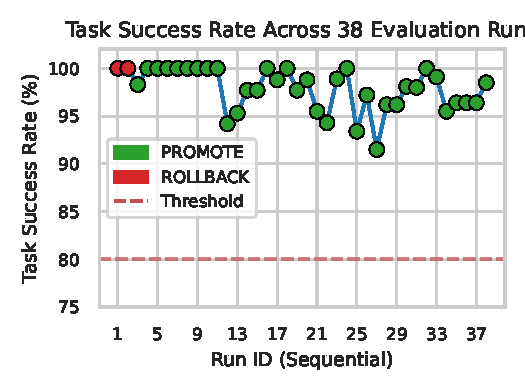
\includegraphics[width=0.9\linewidth]{figures/success_rate.pdf}
\caption{Success rate across 38 evaluation runs. Green markers indicate PROMOTE decisions; red markers indicate ROLLBACK. The dashed line marks the 80\% acceptance threshold.}
\label{fig:success_rate}
\end{figure}

\begin{figure}[ht]
\centering
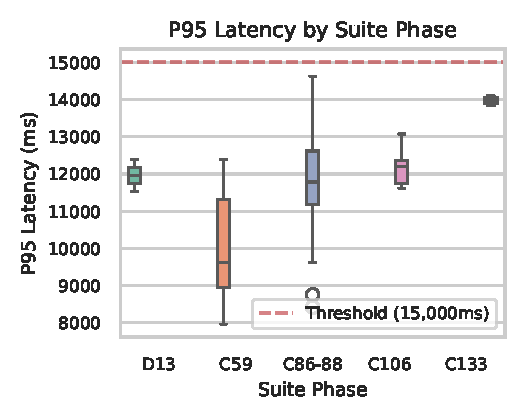
\includegraphics[width=0.9\linewidth]{figures/latency_distribution.pdf}
\caption{Distribution of P95 latency by suite phase labels (D13, C59, C86-88, C106, C133). The increasing trend ($\tau = 0.374$) correlates with growing test-suite complexity.}
\label{fig:latency_distribution}
\end{figure}

\begin{figure*}[t]
\centering
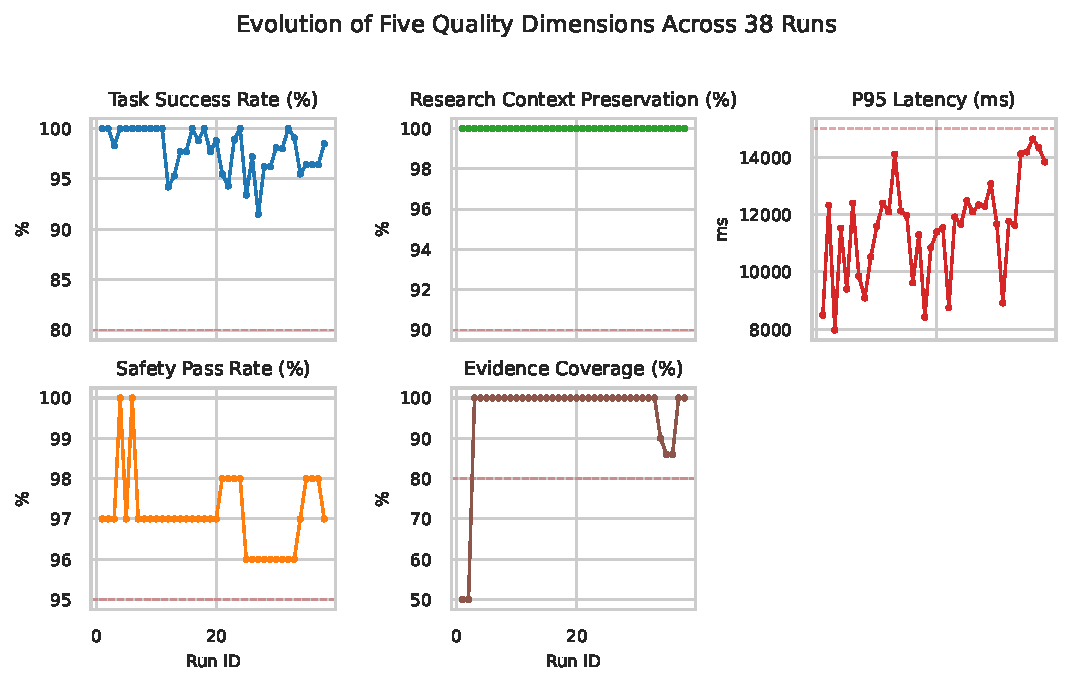
\includegraphics[width=0.98\textwidth]{figures/quality_evolution.pdf}
\caption{Joint evolution of the five gate dimensions across 38 evaluation runs. Task success trend reflects increasing test-suite difficulty; evidence coverage isolates severe regressions; latency growth tracks suite expansion while remaining under threshold.}
\label{fig:quality_evolution}
\end{figure*}

Table~\ref{tab:descriptive} reports descriptive statistics across all runs, complementing the trend and correlation analyses.
\begin{table}[htbp]
\renewcommand{\arraystretch}{1.2}
\centering
\scriptsize
\setlength{\tabcolsep}{2.5pt}
\caption{Descriptive statistics across evaluation runs.}
\label{tab:descriptive}
\begin{tabular}{p{1.35cm}rrrrrr}
\toprule
\textbf{Metric} & \textbf{Mean} & \textbf{Med.} & \textbf{SD} & \textbf{Min} & \textbf{Max} & \textbf{IQR} \\
\midrule
Task Success & 97.9 & 98.4 & 2.2 & 91.5 & 100.0 & 3.6 \\
P95 Latency & 11542.3 & 11715.5 & 1769.3 & 7970.0 & 14631.0 & 1777.2 \\
Research Ctx. Pres. & 100.0 & 100.0 & 0.0 & 100.0 & 100.0 & 0.0 \\
Safety Pass & 97.1 & 97.0 & 1.0 & 96.0 & 100.0 & 0.0 \\
Evidence Coverage & 96.4 & 100.0 & 11.6 & 50.0 & 100.0 & 0.0 \\
\bottomrule
\end{tabular}
\setlength{\tabcolsep}{6pt}
\end{table}


\subsection{Operational Overhead and Scalability}
Beyond quality outcomes, we measured the runtime overhead of the gate itself (Table~\ref{tab:overhead_scaling}). Due to the asymmetric, long-tail distribution typical of LLM generation, median durations provide a more robust metric. The median run duration was approximately 407.3 seconds (min 59.4s, max 801.4s), with a median of 4{,}661.0ms per evaluated test. The relationship between suite size and runtime is strongly linear (Pearson $r=0.92$), with an estimated slope of approximately +6.0 seconds per additional test. This indicates predictable scaling behavior for release planning and CI capacity provisioning.

\begin{table}[htbp]
\renewcommand{\arraystretch}{1.2}
\centering
\scriptsize
\setlength{\tabcolsep}{2.5pt}
\caption{Operational overhead by suite size. Total tests vs run duration: Pearson $r=0.92$ ($p=0.000$), slope $+5996$ ms/test.}
\label{tab:overhead_scaling}
\begin{tabular}{rrrrr}
\toprule
\textbf{Suite} & \textbf{Runs} & \textbf{Med. s} & \textbf{Med./Test ms} & \textbf{P95 ms} \\
\midrule
13 & 2 & 61.1 & 4702.7 & 11960 \\
50 & 1 & 191.9 & 3837.6 & 8915 \\
59 & 9 & 241.1 & 4086.7 & 9850 \\
83 & 3 & 548.5 & 6608.5 & 14331 \\
86 & 9 & 409.6 & 4763.2 & 11393 \\
88 & 4 & 391.0 & 4443.1 & 11604 \\
106 & 8 & 523.4 & 4937.4 & 12194 \\
133 & 2 & 789.4 & 5935.4 & 13974 \\
\bottomrule
\end{tabular}
\setlength{\tabcolsep}{6pt}
\end{table}


These patterns demonstrate the value of treating LLM development as an iterative, empirical process governed by strict quantitative gates, while highlighting that trend interpretation must account for evolving test difficulty.
